\documentclass[tikz,border=2mm]{standalone}
\usepackage{tikz}
\usetikzlibrary{calc,intersections,angles,quotes}
\usepackage{animate}
\begin{document}
%==================
\def\dai{2}
\def\rong{.2}
\def\goc{60}
\pgfmathsetmacro\hs{sqrt(3)}
\def\hh{5}
\def\sfa{180}
%\begin{animateinline}[controls,autoplay,palindrome,loop]{8}
%\multiframe{\sfa}{i=0+1}{
%\foreach \i in {0,1,...,179,180,179,...,0}{
\begin{tikzpicture}
\foreach \x in {0,...,10}{
\foreach \y in {0,1,2}{
\draw[gray!50,fill=gray!80] 
(\x,\y *\hs+\rong *\hs)--++(\goc:\dai)--++(180-\goc:\rong)--++(180+\goc:\dai)--cycle
($(\x,\y *\hs+\rong *\hs)+(180-\goc:\rong)+(\goc:.5*\dai-.5*\rong)$) --++(180-\goc:\dai)--++(\goc:\rong)--++(-\goc:\dai)--cycle
;
}
}
\end{tikzpicture}

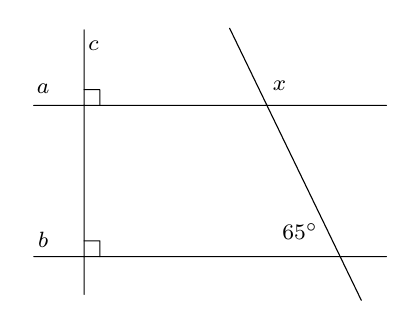
\begin{tikzpicture}[line join = round, line cap = round,>=stealth,font=\footnotesize,scale=.8]
		% Khai báo điểm, xác định các điểm trong hình vẽ
		\def\dodai{0.8}
		\pgfmathsetmacro\a{\dodai}
%		\pgfmathsetmarco{\a}{\dodai};
		\path 
		(0,0) coordinate (b)
		(0,3*\a) coordinate (a)
		($(b)+(7*\a,0)$) coordinate (dpb)
		($(a)+(7*\a,0)$) coordinate (dpa)
		($(b)+(1*\a,0)$) coordinate (M)
		($(b)+(6*\a,0)$) coordinate (N)
		($(M)!0.9!90:(N)$) coordinate (c)
		($(M)!0.15!-90:(N)$) coordinate (dpc)
		($(N)!1!-65:(M)$) coordinate (d)
		($(N)!0.2!185:(d)$) coordinate (dpd)
		(intersection of a--dpa and M--c) coordinate (K)
		(intersection of a--dpa and dpd--d) coordinate (E)
		(intersection of b--dpb and dpd--d) coordinate (F)
		;
		\pgfresetboundingbox
		\draw 
		(a)--(dpa)
		(b)--(dpb)
		(c)--(dpc)
		(d)--(dpd)
		;
		\path 
		pic[angle radius=2mm,"$x$",angle eccentricity=1.5] {angle = dpa--E--d}
		pic[angle radius=4mm,"$65^\circ$",angle eccentricity=1.5] {angle = E--F--b}
		;
		\foreach \x/\y/\z in {c/M/N,c/K/dpa}\pic[draw,angle radius=2mm]{right angle=\x--\y--\z}; % Đánh dấu góc vuông
		%		\foreach \x in {A,B,C,M}\draw[fill=black] (\x) circle (1pt);
		\foreach \x/\g in {a/60,b/60,c/-60}\path ($(\x)+(\g:3mm)$)node{$\x$};
	\end{tikzpicture}


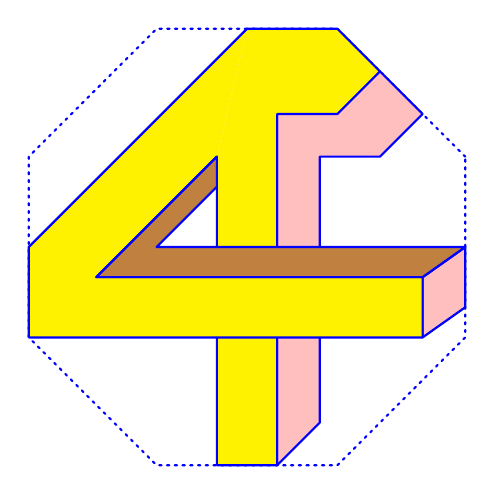
\begin{tikzpicture}[join=round,cap=round,thick,blue]
\def\r{3}
\pgfmathsetmacro\a{\r *cos(67.5)}
\pgfmathsetmacro\b{\a *sqrt(2)}
\pgfmathsetmacro\h{\b+\a}
\draw[dotted] (22.5:\r) \foreach \i in {1,...,7}{--(22.5+45*\i:\r)}--cycle;
\draw[fill=pink]
(\h-\b/3,-\a/3)--(\h,0)--(\h,-2*\a/3)--(\h-\b/3,-\a)--cycle
(\a/3,-\h)--(\a/3+\b/3,-\a-2*\b/3)--(\a/3+\b/3,\a)--(\a+\b/3,\a)--(\h-\b/3,\a+\b/3)--(\a+\b/3,\h-\b/3)--(\a,\h-\b/3)--(\a/3,\h-\b/3)--cycle
;
\draw[fill=yellow] (-\a/3,\a)--(-\a/3,-\h)--(\a/3,-\h)--(\a/3,\a+\b/3)--(\a,\a+\b/3)--++(45:2*\a/3)--++(135:2*\a/3)--(0,\h);
\draw[fill=yellow] (0,\h)--(-\h,0)--(-\h,-\a)--(\h-\b/3,-\a)--(\h-\b/3,-\a/3)--(-5*\a/3,-\a/3)--(-\a/3,\a);
\draw[fill=brown] 
(\h-\b/3,-\a/3)--(\h,0)--(-\a,0)--(-\a/3,2*\a/3)--(-\a/3,\a)--(-5*\a/3,-\a/3)--cycle
;
\end{tikzpicture}

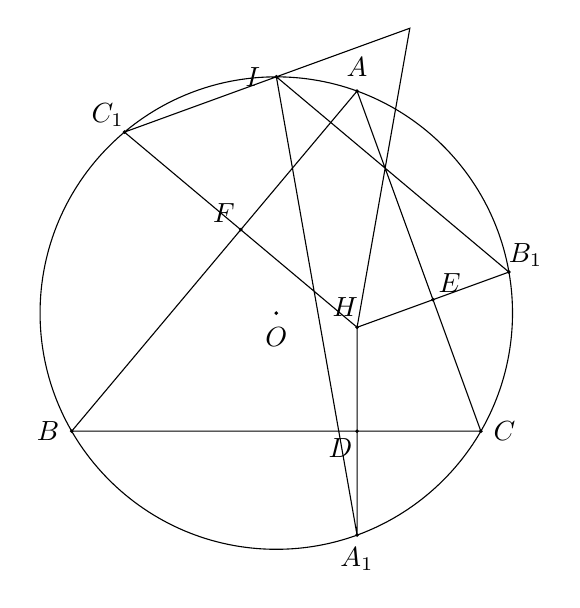
\begin{tikzpicture}
\def\r{3}
\def\gd{80}
\path
(0:0) coordinate (O)
(70:\r) coordinate (A)
(210:\r) coordinate (B)
(330:\r) coordinate (C)
($(B)!(A)!(C)$) coordinate (D)
($(A)!(C)!(B)$) coordinate (F)
($(C)!(B)!(A)$) coordinate (E)
(intersection of A--D and C--F) coordinate (H)
($(H)!2!(D)$) coordinate (A_1)
($(H)!2!(E)$) coordinate (B_1)
($(H)!2!(F)$) coordinate (C_1)
(H)+(\gd:1mm) coordinate (d)
(intersection of H--d and B--C) coordinate (d_1)
(intersection of H--d and A--C) coordinate (d_2)
(intersection of H--d and A--B) coordinate (d_3)
(intersection of A_1--d_1 and C_1--d_3) coordinate (I)
;
\draw
(O) circle (\r)
(A)--(B)--(C)--cycle
(A_1)--(H) (B_1)--(H) (C_1)--(H)
(H)--(d_3)--(C_1)
(I)--(A_1) (I)--(B_1)
;
\foreach \x/\g in {A/90,B/180,C/0,D/-135,E/45,F/135,H/120,A_1/-90,B_1/45,C_1/135,I/180,O/-90}\fill (\x) circle (.025)+(\g:.3)node{$\x$};
\end{tikzpicture}
%}
%\end{animateinline}
\end{document}
%%23:26:29 11/11/2020Last Modification of contents